% SNU_sample.tex v1.0
% 논문작성을 위해서 한글패키지가 설치되어 있어야 합니다.
% MikTeX 을 사용할 것을 권장하며, MikTeX의 설치 및 한글 패키지와 관련된 사항은
% KTUG 한글 TeX 사용자 그룹 http://www.ktug.or.kr을 참조하시길 바랍니다.
%
% 본 tex file의 여백은 B5(JIS)에 맞춰져 있습니다.
% 컴파일을 완료하고 ps file을 생성한뒤, command prompt에서
% dvips -T 182mm,257mm -o Snu_sample.ps Snu_sample.dvi명령어를
% 사용하여 .ps file을 생성하면 됩니다.
%
% ps file을 pdf로 변환한 뒤에, 인쇄시 B5(JIS)에 맞춰서 출력하고,
% 옵션중 페이지 비율을 없음으로 해야 원하는 여백 그대로 출력됩니다.
%

% SNU_template.cls file을 사용합니다.
% 박사의 경우 \documentclass[doctor]{SNU_template} (default)
% 석사의 경우 \documentclass[master]{SNU_template} 로 변경하면 됩니다.
% SNU_template.cls file명이 바뀔경우에는 {SNU_template} 대신에 {바뀐 file명}을 넣으면 됩니다.
% 주어진 .cls file의 내용을 변경하는 것은 규격에 어긋난 결과를 낼 수 있습니다.
%
% 주어진 .cls file은 서울대학교 논문 규격에 맞춰서 작성되어 있으며,
% MS Word 양식과 동일한 output을 내도록 작성되어 있으므로
% 특별한 설명이 없는 부분은 Word양식의 guideline을 참조하시면 됩니다.

\documentclass[master,korean]{snuee}

%

% 논문 작성을 위한 사전 준비과정
% 논문제목 (국문, 영문), 저자, 제출일, 심사일, 졸업일의 정보를 넣습니다.

% 논문제목을 넣습니다.
% 필히 한글제목과 영문제목 모두 넣어야 합니다.
\title[korean]{논 문 제 목}
\title[english]{TITLE OF THE THESIS}

% 저자 정보를 넣습니다.
% 국문성명, 영문성명 모두 넣어야 하며, 특히 국문성명의 경우는 글자사이에 space가 있는 것과 없는 것
% 두 가지 모두를 집어넣어줘야 합니다.
\author[korean]{홍 길 동}
\author[english]{HONG GIL-DONG}
\author[nospace]{홍길동}

% 지도교수님의 성함을 국문으로 넣습니다.
\adviser{홍 길 몽}

% 논문 제출일, 논문 심사일을 한글로 넣습니다.
\submissiondeadline{2007년 4월} \examinationdate{2007년 6월}

% 졸업일을 영문식, 한글식 두 가지 방법 모두 넣습니다.
\gradyear[english]{AUGUST 2007} \gradyear[korean]{2007년 8월}

%

% 문서의 시작
%
% 위의 정보들을 빠짐없이 채워넣고 document를 시작하면
% 외표지, 내표지(외표지와 동일), 인준지가 자동으로 생성됩니다.

\begin{document}
\renewcommand{\baselinestretch}{1.5}    % 본문의 줄간격 조정, 고치거나 삭제하지 마십시오.
\selectfont                             %

% abstract(영문)의 작성
% begin과 end 사이에 abstract의 내용을 채워넣습니다.
    \begin{abstract}
    \par %abstract 첫 문장 들여쓰기, 고치거나 삭제하지 마십시오.
    이 텍 파일은 SNU EECS의 논문양식 샘플입니다.
    용지는 B5(JIS:182mm$\times$257mm)으로 의도되었으며,
    영문 글자체는 Times New Roman, 한글 글자체는 명조체로 되어 있습니다.
    여백이나 줄간격 등은 워드 양식의 Description.doc를 참고하세요.

% abstract page 하단에 keyword와 학번을 넣습니다.
    \vfill
    \begin{minipage}[t][20mm][b]{\textwidth}
    {\bfseries 주요어}: SNU template, TeX\\
    {\bfseries 학 번}: 2007-2007\\
    \end{minipage}

    \end{abstract}

    %\changepage{5mm}{}{}{}{}{}{}{}{-5mm}    %%페이지 여백 재설정. 절대 고치거나 삭제하지 마십시오.
    \makelists   %목차를 자동생성합니다.


% 본문의 시작
% chapter, section의 추가,변경등 모두를 자유롭게 할 수 있습니다.
% 그림, 표의 추가 형식은 MS Word의 형식과 동일합니다. (MS Word Description file 참조)
%
    \chapter{INTRODUCTION}
    This is LaTeX version of the SNU thesis template. Page margins, font size are already applied in SNU\_sample.cls.
    So, you can just put your texts at here and compile it, you can
    obtain your own thesis file.
    You can freely remove sample chapters and add your own chapters,
    sections, subsections, figures and so on.
    \\
    \\
    \\
    These are examples of making section and subsection.
    We'll show you other examples of putting your figures and
    tables.

	\section{제목}
	내용으로 꽉 채워서 페이지 번호 여백이 적절한지 체크해야 됨.
	내용으로 꽉 채워서 페이지 번호 여백이 적절한지 체크해야 됨.
	내용으로 꽉 채워서 페이지 번호 여백이 적절한지 체크해야 됨.
	내용으로 꽉 채워서 페이지 번호 여백이 적절한지 체크해야 됨.
	내용으로 꽉 채워서 페이지 번호 여백이 적절한지 체크해야 됨.
	내용으로 꽉 채워서 페이지 번호 여백이 적절한지 체크해야 됨.
	내용으로 꽉 채워서 페이지 번호 여백이 적절한지 체크해야 됨.
	내용으로 꽉 채워서 페이지 번호 여백이 적절한지 체크해야 됨.
	내용으로 꽉 채워서 페이지 번호 여백이 적절한지 체크해야 됨.
	내용으로 꽉 채워서 페이지 번호 여백이 적절한지 체크해야 됨.
	내용으로 꽉 채워서 페이지 번호 여백이 적절한지 체크해야 됨.
	내용으로 꽉 채워서 페이지 번호 여백이 적절한지 체크해야 됨.
	내용으로 꽉 채워서 페이지 번호 여백이 적절한지 체크해야 됨.
	내용으로 꽉 채워서 페이지 번호 여백이 적절한지 체크해야 됨.
	내용으로 꽉 채워서 페이지 번호 여백이 적절한지 체크해야 됨.
	내용으로 꽉 채워서 페이지 번호 여백이 적절한지 체크해야 됨.
	내용으로 꽉 채워서 페이지 번호 여백이 적절한지 체크해야 됨.
	내용으로 꽉 채워서 페이지 번호 여백이 적절한지 체크해야 됨.
	내용으로 꽉 채워서 페이지 번호 여백이 적절한지 체크해야 됨.
	내용으로 꽉 채워서 페이지 번호 여백이 적절한지 체크해야 됨.
	내용으로 꽉 채워서 페이지 번호 여백이 적절한지 체크해야 됨.
	내용으로 꽉 채워서 페이지 번호 여백이 적절한지 체크해야 됨.
	내용으로 꽉 채워서 페이지 번호 여백이 적절한지 체크해야 됨.
	내용으로 꽉 채워서 페이지 번호 여백이 적절한지 체크해야 됨.
	내용으로 꽉 채워서 페이지 번호 여백이 적절한지 체크해야 됨.
	내용으로 꽉 채워서 페이지 번호 여백이 적절한지 체크해야 됨.
	내용으로 꽉 채워서 페이지 번호 여백이 적절한지 체크해야 됨.
	내용으로 꽉 채워서 페이지 번호 여백이 적절한지 체크해야 됨.
	내용으로 꽉 채워서 페이지 번호 여백이 적절한지 체크해야 됨.

    \section{Section Example}
    This is section example.
    \subsection{Subsection Example}
    This is subsection example.

    \chapter{FIGURES AND TABLES}
    \section{Figures}
    This section shows how to insert your figures in your thesis.\\
    \begin{figure}[htbp]
    {
    \begin{center}
    \begin{tabular}{c}
	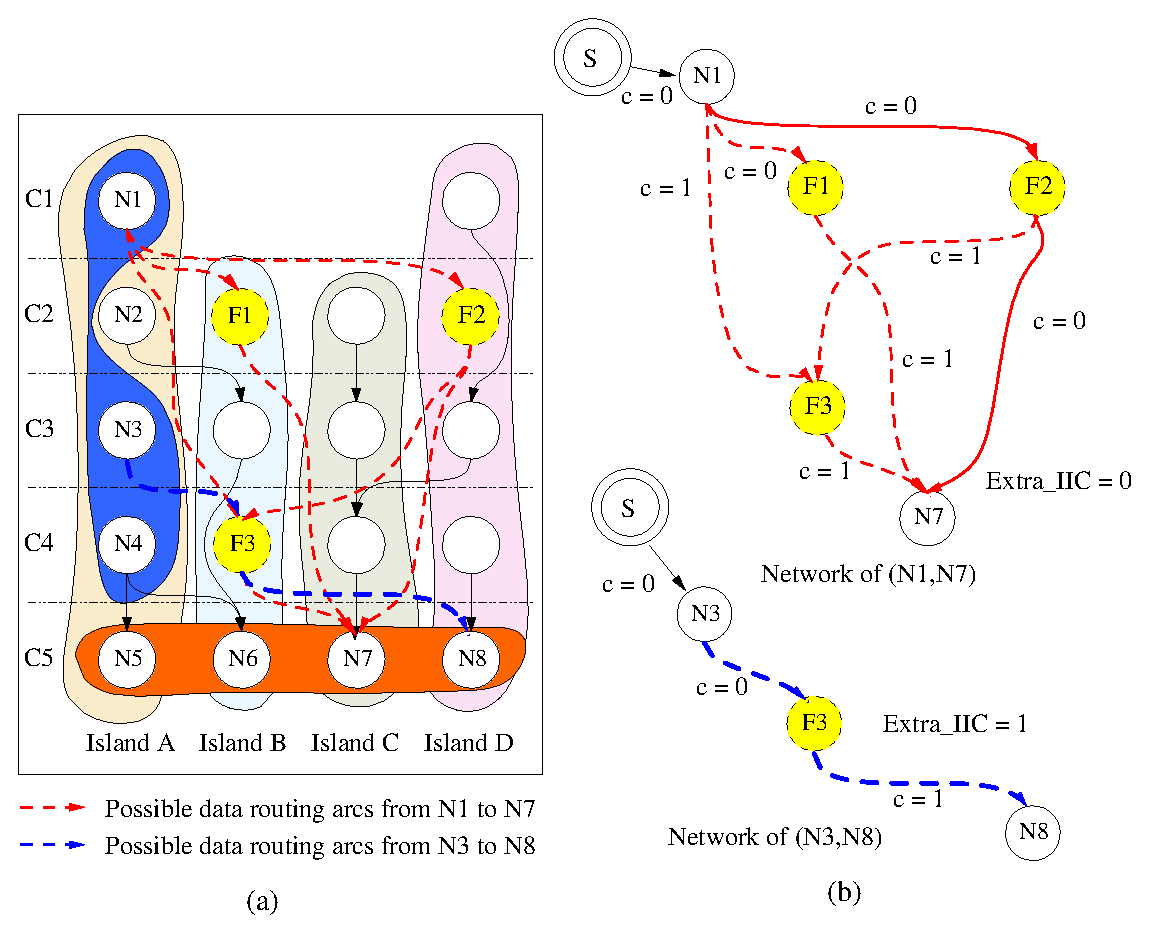
\includegraphics[height=6cm]{Sample.eps}
    \end{tabular}
    \end{center}
    }
    \caption{Example 1.}
    \end{figure}\\
    The caption of the figure should be located below the figure and end with '.'
    \subsection{subsection test}
    test1

    \subsubsection{subsubsection test}
    test2

    \newpage
    If the caption of the figure is longer than one lines, you should
    align it left.(This is default)\\

    \begin{figure}[htbp]
    {
    \begin{center}
    \begin{tabular}{c}
	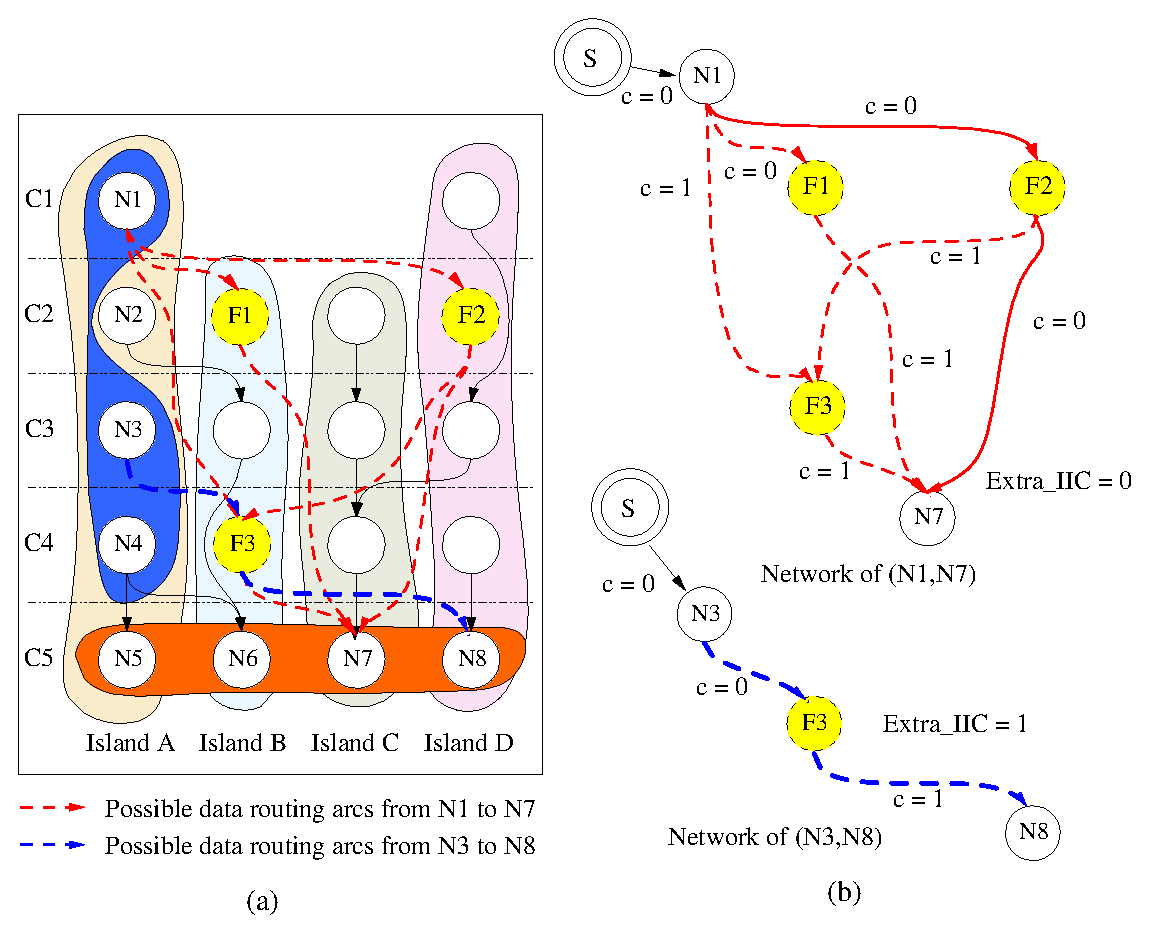
\includegraphics[height=6cm]{Sample.eps}
    \end{tabular}
    \end{center}
    }
    \caption{The second example - Access conflict and an extended
data-forwarding scheme. }
    \end{figure}
    \newpage

    \section{Tables}
    This is example of inserting your tables in your thesis. The
    caption of the table should be located above the table. Be
    careful that caption should not end with '.'
    \begin{table}[htbp]
    \begin{center}
    \caption{Example 3} \label{tab1}
    \begin{tabular}{|c|c|c|} \hline
    Benchmarks & Number of nodes  & L\\ \hline
    \hline {\sc chen} & 87  & 14\\ \hline {\sc 3d\_force1} & 53  & 15\\
    \hline {\sc 3d\_force2} & 36  & 11\\ \hline {\sc 3d\_motion} & 45  &
    6\\ \hline {\sc mpeg\_calcid} & 27  & 8\\ \hline {\sc adpcm\_dec} &
    15  & 6 \\ \hline {\sc jm\_itrans} & 58  & 9\\ \hline {\sc 4ar} & 28
    & 8\\ \hline
    \end{tabular}
    \end{center}
    \end{table}

%
% 참고문헌을 넣습니다.
% 샘플의 형식과 같은 차례대로 써줍니다.
%

%

\begin{thebibliography}{00}

% 영문저널의 경우
    \bibitem{ref1} B. Jeon and J. Jeong, ``Blocking artifacts
    reduction in image compression with block boundary discontiunity
    criterion,'' {\em IEEE Transactions on Circuits and Systems for
    Video Tech.}, vol. 8, no.3, pp. 345-357, June 1998.

% 영문학술대회의 경우
    \bibitem{ref2} W. G. Jeon and Y. S. Cho, ``An equalization
    technique for OFDM and MC-CDMA in a multipath fading channels,''
    in {\em Proceedings of IEEE Conference on Acoustics, Speech and
    Signal Processing}, Munich, Germany, May 1997. pp. 2529-2532.

% 국내저널의 경우
    \bibitem{ref3} 김남훈, 정영철, ``평탄한 통과대역 특성을 갖는
    새로운 구조의 광도 파로열 격자 라우터,'' {\em 전자공학회논문지},
    제35권 D편, 제3호, 56-62쪽, 1998년 3월.

% 국내학술대회의 경우
    \bibitem{ref4} 윤남국, 김수종, ``무선 센서 네트워크에서의 에너지
    효율적인 그라디언트 기반 라우팅 기법,'' {\em 한국정보과학회
    2006년 추계학술대회}, 제12권, 제2호, 2006년 10월. pp.
    1372-1374.

% 단행본의 경우
    \bibitem{ref5} C. Mead and L. Conway, {\em Introduction to VLSI
    Systems}, Addison-Wesley, Boston, 1994.

% URL
    \bibitem{ref6} The SolarMESH Network,
    http://owl.mcmater.ca/solarmesh

% Technical Report의 경우
    \bibitem{ref7} K. E. Elliott and C. M. Greene, ``A local adaptive
    protocol,'' Argonne National Laboratory, Argonne, France,
    Technical Report 916-1010-BB, 1997.

% 학위논문의 경우
    \bibitem{ref8} T. Kim, ``Scheduling and Allocation Problems in
    High-level Synthesis,'' Ph. D. Dissertation, ECE Department,
    Univ. of Illinois at U-C, 1993.

% 특허의 경우
    \bibitem{ref9} Sunghyun Choi, ``Wireless MAC protocol based on a
    hybrid combination of slot allocation, token passing, and
    polling for isochronous traffic,'' U.S. Patent No. 6,795,418,
    September 21, 2004.

% 표준
    \bibitem{ref10} IEEE Std. 802.11-1999, Part 11: Wireless LAN
    Medium Access Control (MAC) and Physical Layer (PHY)
    specifications, Reference number ISO/IEC 8802-11:1999(E), IEEE
    Std. 802.11, 1999 edition, 1999.

\end{thebibliography}

%---------------------------------------------------------------------------------
% 본문의 종료
% 국문 초록과 감사의 글(선택)을 넣습니다.
% begin{summary}와 end{summary}의 사이에 국문초록을 집어넣습니다.
% 감사의글은 \acknowledgement{}의 대괄호 안에 내용을 넣습니다.
%
    \begin{summary}
    \par    %첫 줄 들여쓰기를 위한 단락구분.삭제하지 마십시오.
    Put your abstract in Korean.
    \vfill
    \begin{minipage}[t][20mm][b]{\textwidth}
    {\bfseries 주요어}: 서울대학교 논문양식, TeX\\
    {\bfseries 학번}: 2007-2007\\
    \end{minipage}
    \end{summary}
    %\changepage {5mm}{}{}{}{}{}{}{}{5mm} %초록과 감사의 글을 위한 여백 재설정, 고치거나 삭제하지 마십시오.
    \acknowledgement{
                        \par
                        Put your acknowledgement here.(optional)} %감사의 글을 작성하지 않을경우 삭제가능
\end{document}
